\documentclass{article}



% Language setting

% Replace `english' with e.g. `spanish' to change the document language

\usepackage[english]{babel}



% Set page size and margins

% Replace `letterpaper' with `a4paper' for UK/EU standard size

\usepackage[letterpaper,top=2cm,bottom=2cm,left=3cm,right=3cm,marginparwidth=1.75cm]{geometry}



% Useful packages

\usepackage{amsmath}

\usepackage{amssymb}

\usepackage{graphicx}

\usepackage[colorlinks=true, allcolors=black]{hyperref}

\usepackage{titlesec}
\usepackage{xparse}



\NewDocumentCommand{\qcq}{m o o m}{%
	\ensuremath{\forall #1 \IfValueT{#2}{, #2} \IfValueT{#3}{, #3}  \in  \mathbb{#4}}%
}
\NewDocumentCommand{\ext}{m o o m}{%
	\ensuremath{\exists #1 \IfValueT{#2}{, #2} \IfValueT{#3}{, #3}  \in  \mathbb{#4}}%
}



\title{\textbf{Rappels et compléments de calcul}}

\author{\textbf{Yassin Akkab}}



\newcommand{\R}{\mathbb{R}}
\newcommand{\N}{\mathbb{N}}
\newcommand{\Z}{\mathbb{Z}}
\newcommand{\C}{\mathbb{C}}
\newcommand{\Q}{\mathbb{Q}}
\newcommand{\D}{\mathbb{D}}





\graphicspath{ {./Screenshots/} }




\begin{document}
	
	\maketitle
	
	
	
	\tableofcontents
	
	\newpage
	
	\section{Les ensembles de nombres usuels}
	\subsection{Définition}
	On définit les ensembles de nombres suivants : 
	\begin{enumerate}
		\item $ \mathbb{N} = \{0, 1, 2, 3, \ldots\} $ l'ensemble des entiers naturels ;
		\item $ \mathbb{Z}= \N \cup -\N  = \{\dots,-2,-1,0,1,2,\dots \} $ l'ensemble des entiers relatifs ;
		\item $\Q = \{\frac{p}{q} | p,q \in \Z, q \neq 0\} $
		\item $\R$ l'ensemble des abscisses d'une droite graduée, l'ensemble des réels;
		\item $\C$ l'ensemble nombres de la forme $a+ib$ ou a,b $\in$ $\R$ et $i^2 = -1$, l'ensemble des complexes.
		
	\end{enumerate}

	Et on note $\N^*, \Q^*,\R^*, \C^*$ les memes ensembles privés de 0.
	
	L'ensemble $\R \backslash \Q$ est appelé l'ensemble des irrationnels.
	
	On considère parfois aussi l'ensemble $\D$ des nombres décimaux : $\D$ = \{$\frac{n}{10^m}|n,m \in \Z$ \}

	\begin{figure}[h]
		\centering
		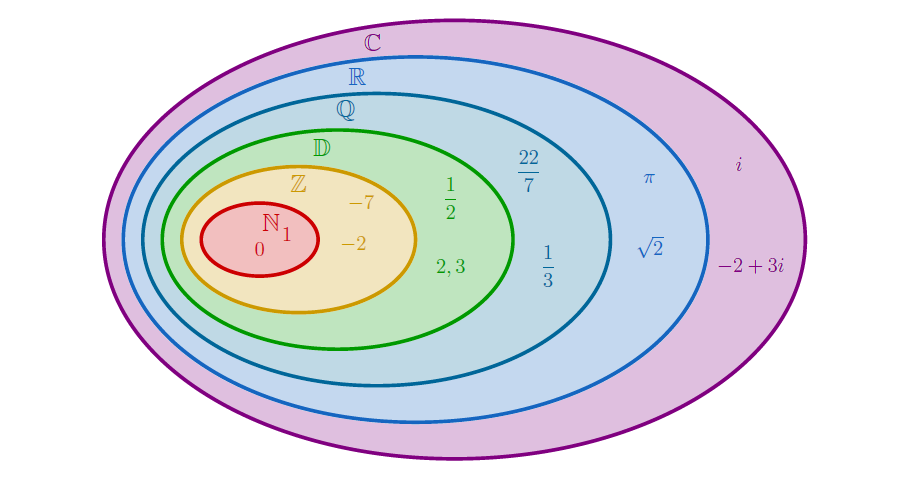
\includegraphics[width=0.7\textwidth]{image1.png}
	\end{figure}
\end{document}